\documentclass[11pt,a4paper]{article}
\usepackage[a4paper,margin=2.5cm]{geometry}
\setlength{\emergencystretch}{3em}
\usepackage{graphicx}
\usepackage{booktabs}
\usepackage{amsmath}
\usepackage{xcolor}
\usepackage{caption}
\usepackage[hidelinks]{hyperref}

\graphicspath{{figures/}}
\captionsetup{font=small,labelfont=bf}

\title{\textbf{Cache Optimisations and CSR Sparse Storage for Dense Matrix
Multiplication:\\ A Controlled Benchmarking Study}}
\author{Alejandro Delgado Valera\\
\small BIG DATA -- Individual Assignment 2\\
\small Grado en Ciencia e Ingenier{\'i}a de Datos\\
\small Universidad de Las Palmas de Gran Canaria\\
\small \url{https://github.com/aledelgadoo/individual-assignments-bigdata}}
\date{October 20, 2026}

\begin{document}
\maketitle

\begin{abstract}
\noindent\textbf{Questions:} (A) how do loop reordering and cache blocking affect
the runtime and memory of dense $O(n^3)$ multiplication relative to a validated
triple-loop baseline, and (B) under which tested sparsity levels does a CSR sparse
representation beat dense methods on matched logical inputs, once conversion costs
are measured separately? All four methods are single-threaded C kernels
(\texttt{float64}, flags \texttt{-O2 -std=c11}) with bitwise-identical results,
measured on the multiplication kernel with warm-ups, five batched repetitions and a
declared budget of 60\,s and 4\,GiB. Loop reordering to \texttt{ikj} yields
2.5--2.8$\times$ over the \texttt{ijk} baseline at $n \in \{500,1000\}$ and
7.0$\times$ at $n=2000$; cache blocking with tile size 64 is slower than
\texttt{ikj} up to $n=1000$ but 1.6$\times$ faster at $n=2000$, where the
32\,MB $B$ matrix no longer fits in the 12\,MB last-level cache. Dense runtimes are
flat across sparsity levels; CSR time falls monotonically from 263\,ms (1\,\% zeros)
to 4.0\,ms (99\,\% zeros) at $n=1000$, beating every dense method on the whole
tested grid, while dense-to-CSR conversion (1.4--10.7\,ms) amortises within one
multiplication. Peak resident memory grows from 26.7\,MB (dense) to 38.1\,MB (CSR)
at $n=1000$. Conclusions are scoped to these kernels, this machine and uniformly
random sparsity.
\end{abstract}

\section{Introduction and objective}

Assignment~1 established the baseline for this study: a straightforward
$i$--$j$--$k$ dense multiplication whose constant factors are dominated by memory
behaviour rather than by the $2n^3$ arithmetic once the matrices leave
cache~\cite{strang2016,cormen2022}. This assignment asks which cheap, purely local
changes improve that baseline, and whether a sparse storage format pays off when
most entries of $A$ are zero.

\textbf{Research questions.}
\begin{enumerate}
  \item[A:] How do loop reordering (\texttt{ikj}) and cache blocking (\texttt{block})
        affect dense multiplication time and memory relative to the validated
        \texttt{ijk} baseline, under one controlled protocol?
  \item[B:] Under which tested sparsity levels does a CSR sparse implementation
        outperform the dense methods on matched logical inputs, with conversion
        costs measured separately?
\end{enumerate}

\textbf{Hypotheses (stated before measurement).}
\begin{enumerate}
  \item[H1:] \texttt{ikj} is faster than \texttt{ijk} because its inner loop
        streams $B$ by rows instead of by strided columns; the advantage grows
        with $n$ as strided access stresses the TLB and caches.
  \item[H2:] Blocking pays off only when the working set exceeds the last-level
        cache; at small and medium $n$ its bookkeeping makes it no faster than
        \texttt{ikj}.
  \item[H3:] The dense methods do not get faster with sparsity: skipping zeros is
        not what the dense loops do.
  \item[H4:] CSR time tracks the number of nonzeros, so it decreases with
        sparsity and crosses below the best dense method at some tested level.
  \item[H5:] All four methods produce bitwise-identical results on matched
        inputs, because they share one summation order.
\end{enumerate}

The controlled factor is the method; the outcome measures are kernel time per
multiplication, peak resident memory, and (for CSR) conversion time.

\section{Background}

\textbf{Loop order and memory access.} In row-major storage the baseline
\texttt{ijk} loop reads $B$ down columns with stride $8n$ bytes, which destroys
spatial locality and stresses the TLB at large $n$. The reordered \texttt{ikj}
loop traverses $B$ by rows (contiguous 64-byte lines) and accumulates into a
contiguous row of $C$, trading a read-modify-write of $C$ for streaming accesses
everywhere~\cite{golub2013,cormen2022}. Both perform the same $2n^3$ FLOPs in the
same $k$ order, so their floating-point results are bitwise equal~\cite{isoC11}.

\textbf{Cache blocking.} Blocking partitions the $k$ loop into tiles of width $B$
so that the $B \times B$ tiles of $A$, $B$ and $C$ stay resident while reused.
The tile working set is roughly $3 \times 8B^2$ bytes: 24\,KB at $B=32$ (fits the
48\,KB L1d) and 98\,KB at $B=64$ (fits the 1.25\,MB L2). The optimal tile is a
compromise between those levels; we select it empirically instead of assuming one
value~\cite{golub2013}.

\textbf{Compressed sparse row (CSR).} CSR stores the nonzeros of $A$ in three
arrays: \texttt{rowptr} ($n{+}1$ indices), \texttt{colind} ($nnz$ column indices)
and \texttt{vals} ($nnz$ values). Multiplying $C = AB$ then loops over the nonzeros
of each row of $A$ and streams the corresponding dense rows of $B$ and
$C$~\cite{saad2003}. The arithmetic work becomes $2 \cdot nnz \cdot n$ instead of
$2n^3$, at the price of storage that can exceed $8n^2$ when $A$ is dense and of a
one-off conversion from the dense input.

\textbf{Benchmarking practice.} We keep the median/IQR summary, the raw
measurements, the single timing boundary and the controlled environment of
Assignment~1~\cite{fleming1986,mytkowicz2009}. One additional laptop-specific
control appears in Section~3: the CPU frequency policy (Section~5).

\section{Methodology}

\subsection{Implementations}

Four single-threaded C11 kernels in one binary (\texttt{src/matmul2.exe}),
compiled with the fixed flags \texttt{-O2 -std=c11 -Wall -Wextra} (GCC 16.1.0,
MinGW-w64); no numerical library runs inside the kernel and all four are
sequential:

\begin{itemize}
  \item \textbf{\texttt{ijk}} -- the Assignment~1 baseline kernel, reused
        unchanged from Git tag \texttt{assignment-1}
        (\texttt{src/c/matmul.c}); validated in that study against NumPy and the
        other languages.
  \item \textbf{\texttt{ikj}} -- same arithmetic, reordered loops so the inner
        \texttt{j} loop streams $B$ by rows; \texttt{restrict} pointers.
  \item \textbf{\texttt{block}} -- tiled $i$/$j$ loops over $k$-tiles of width
        $B \in \{16,32,64,128\}$, selected per $n$ by a tuning sweep
        (Section~4); 64 won at every tuned size.
  \item \textbf{\texttt{csr}} -- dense-to-CSR conversion (two-pass with a cursor
        array), then CSR$\times$dense: for each row of $A$, each nonzero
        \texttt{(k, val)} streams row $k$ of $B$ into row $i$ of $C$.
\end{itemize}

Every kernel zeroes $C$ inside its timed region (the operation includes writing
the output), uses \texttt{float64} arithmetic, and visits $k$ in ascending order,
so all four emit bitwise-identical results on matched inputs (verified in
Section~3.3). Input loading, allocation, conversion (CSR) and checksums are
outside the timed region. The process is pinned to logical CPU0 (a P-core of the
hybrid i7-1355U) with \texttt{SetThreadAffinityMask}.

\subsection{Inputs}

Dense Part~A reuses the Assignment~1 input pairs byte-for-byte. For each
declared size $n = 10$, $50$, $100$, $200$, $500$, $1000$ and $2000$, $A$ and
$B$ were generated with NumPy
PCG64 seed scheme \texttt{default\_rng([42, n, index])}, uniform in $[-1,1)$,
stored as little-endian \texttt{<f8} row-major files, with SHA-256 checksums in
\texttt{data/inputs/meta.json}.

Sparse Part~B keeps $n=1000$ and $B$ dense, and varies only $A$: nine sparsity
levels $p \in \{1,5,10,25,50,75,90,95,99\}$\,\% of zeros, produced by masking
the dense $A_{1000}$ with an independent keep-mask
(\texttt{default\_rng([42, n, p, 2])}, keep if uniform $\ge p/100$), so the
nonzero distribution is uniform random and the same file feeds all four methods.
Recorded nonzero counts match the targets (e.g.\ $nnz = 499\,827$ at 50\,\%,
$9\,844$ at 99\,\%).

\subsection{Correctness}

Before any benchmarking, the self-test executable
(\texttt{matmul2.exe selftest}) ran 304 checks, all passing: sizes $1$--$64$
crossed with four matrix patterns (dense random, 50\,\% zeros, zero matrix,
identity) and four block sizes $\{4,7,16,64\}$; each method was compared against
a \texttt{long double} reference ($rtol = 10^{-10}$, $atol = 10^{-12}$, tight
because the summation orders are identical), bitwise between methods, plus manual
$nnz$ counts and hand-computed $2\times2$/$3\times3$ answers. Independently, the
campaign CSVs show one unique checksum per matched input across the four methods
for all 16 $(n, p)$ groups.

\subsection{Environment}

\begin{center}
\small
\begin{tabular}{@{}ll@{}}
\toprule
CPU & 13th Gen Intel Core i7-1355U, 10 physical / 12 logical processors \\
Cache & L1d 48\,KB per P-core, L2 6656\,KB total, L3 12288\,KB, line 64\,B \\
RAM / OS & 16.8\,GB, Windows 10 (build 26200) \\
Compiler & GCC 16.1.0 (MinGW-w64), \texttt{-O2 -std=c11 -Wall -Wextra} \\
Power scheme & Windows \emph{High performance} (turbo clocks held) \\
Affinity & children pinned to logical CPU0 via \texttt{SetThreadAffinityMask} \\
\bottomrule
\end{tabular}
\end{center}

The first campaign ran under the default \emph{Balanced} plan and was discarded:
single-core frequency oscillated between turbo and throttled states, producing
5$\times$ swings inside one configuration. All reported numbers come from a
re-run under \emph{High performance}; the effect itself is discussed in
Section~5.

\subsection{Measurement protocol}

Identical to Assignment~1, with one binary: monotonic \texttt{QueryPerformanceCounter}
timing of the kernel only; a feasibility probe (one excluded warm-up + one timed
kernel, retried once, gate = timed $\le$ 60\,s); then, for passing configurations,
one excluded warm-up followed by five measured repetitions, batched so each
timing spans at least 0.2\,s (batch sizes calibrated at run time; very slow
kernels use batch $=1$). Summaries are the median and IQR of the five
per-multiplication times. Memory is the peak resident (working-set) size of the
child process, sampled every 50\,ms by the orchestrator (psutil on Windows) and by
the process itself (\texttt{GetProcessMemoryInfo}); budget 4\,GiB. CSR conversion
is timed in its own CSV rows (\texttt{conversions.csv}), never inside the
multiplication timing. System CPU utilisation is recorded per configuration as a
noise covariate. Raw data live in
\texttt{data/results/\{raw\_timings,configs,conversions,blocksize\_tuning\}.csv}.

\section{Results}

All 57 configurations (21 dense + 36 sparse) completed within budget; there are
no timeouts to report. Across configurations the IQR is a median of 4.3\,\% of the
median (maximum 17.8\,\%, on the sub-millisecond $n=200$--$1000$ configurations).

\subsection{Part A: dense optimisation}

\begin{table}[t]
\centering
\caption{Part A: median kernel time per multiplication (ms) over 5 repetitions;
IQR as a percentage of the median ranged 0.2--17.8\,\% (median 4.3\,\%).}
\label{tab:partA}
\small
\begin{tabular}{@{}rrrr@{}}
\toprule
$n$ & \texttt{ijk} & \texttt{ikj} & \texttt{block} ($B=64$) \\
\midrule
10    & 0.0004 & 0.0005 & 0.0005 \\
50    & 0.033  & 0.023  & 0.039 \\
100   & 0.300  & 0.213  & 0.340 \\
200   & 3.22   & 1.84   & 2.85 \\
500   & 75.07  & 29.55  & 41.54 \\
1000  & 806.9  & 286.1  & 325.2 \\
2000  & 27\,478 & 3\,941 & 2\,525 \\
\bottomrule
\end{tabular}
\end{table}

Table~\ref{tab:partA} and Figure~\ref{fig:runtime} show the scaling.
\texttt{ikj} is faster than the baseline from $n=50$ upward: 2.54$\times$ at
$n=500$, 2.82$\times$ at $n=1000$ and 6.97$\times$ at $n=2000$. Blocking follows
a different curve: it is slower than \texttt{ikj} at every size up to $n=1000$
(e.g.\ 1.41$\times$ slower at $n=500$) but overtakes it at $n=2000$, where it is
1.56$\times$ faster than \texttt{ikj} and 10.9$\times$ faster than the baseline
(Figure~\ref{fig:speedup}). The local growth exponent between $n=500$ and
$n=2000$ is 4.26 for \texttt{ijk}, 3.53 for \texttt{ikj} and 2.96 for
\texttt{block}: the baseline is strongly super-cubic, and blocking is the only
method close to the algorithmic $n^3$ at the top end.

\begin{center}
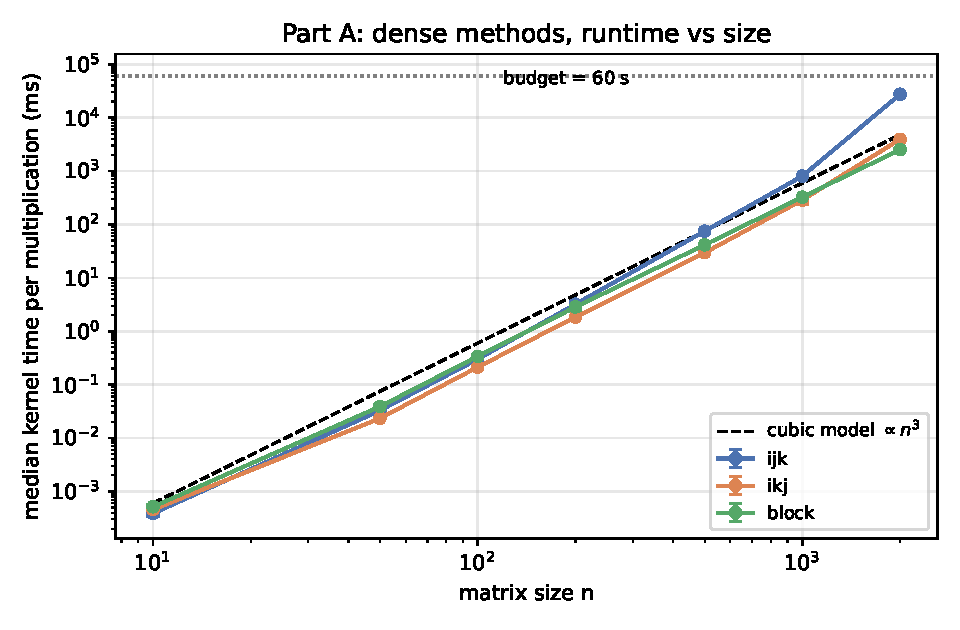
\includegraphics[width=0.82\textwidth]{fig1_runtime_loglog.pdf}
\captionof{figure}{Part A: median kernel time vs.\ $n$ (log-log) with IQR error
bars and a cubic reference anchored at the baseline ($n=500$). All
configurations met the 60\,s budget.}
\label{fig:runtime}
\end{center}

\begin{center}
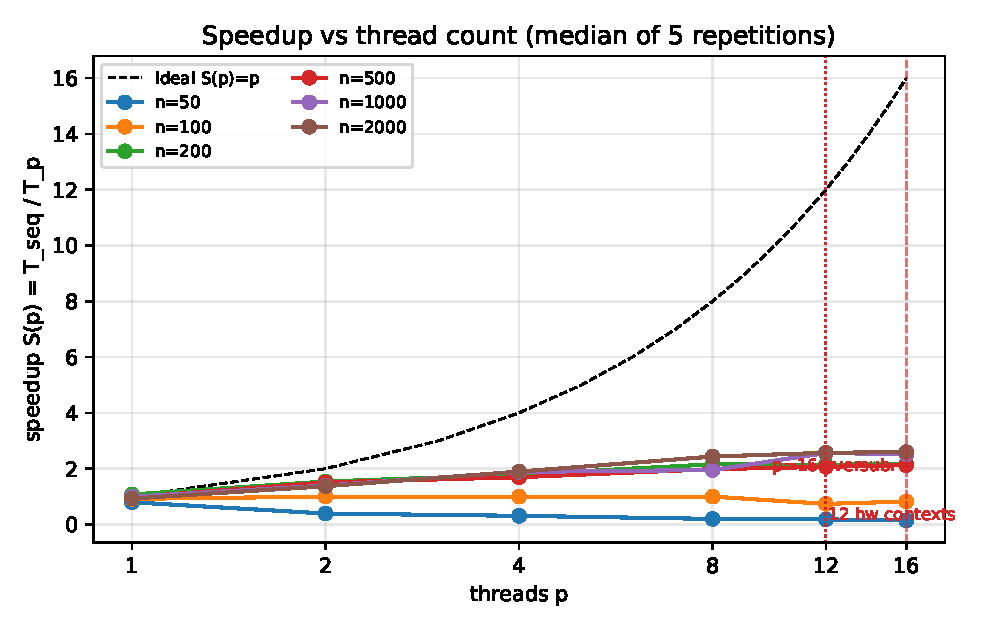
\includegraphics[width=0.78\textwidth]{fig2_speedup.pdf}
\captionof{figure}{Part A: speedup of the optimised methods over \texttt{ijk}
(median times). Blocking only pays off past $n=1000$.}
\label{fig:speedup}
\end{center}

The block size was chosen by a tuning sweep (Table~\ref{tab:tune});
$B=64$ won at every tuned size and was used in the campaign.

\begin{table}[t]
\centering
\caption{Tuning sweep: median kernel time (ms) for four candidate block sizes.}
\label{tab:tune}
\small
\begin{tabular}{@{}rrrrr@{}}
\toprule
$n$ & $B=16$ & $B=32$ & $B=64$ & $B=128$ \\
\midrule
500  & 80.8  & 85.1  & \textbf{46.7} & 57.7 \\
1000 & 960   & 596   & \textbf{313}  & 430 \\
2000 & 11\,377 & 7930 & \textbf{2627} & 3691 \\
\bottomrule
\end{tabular}
\end{table}

\begin{center}
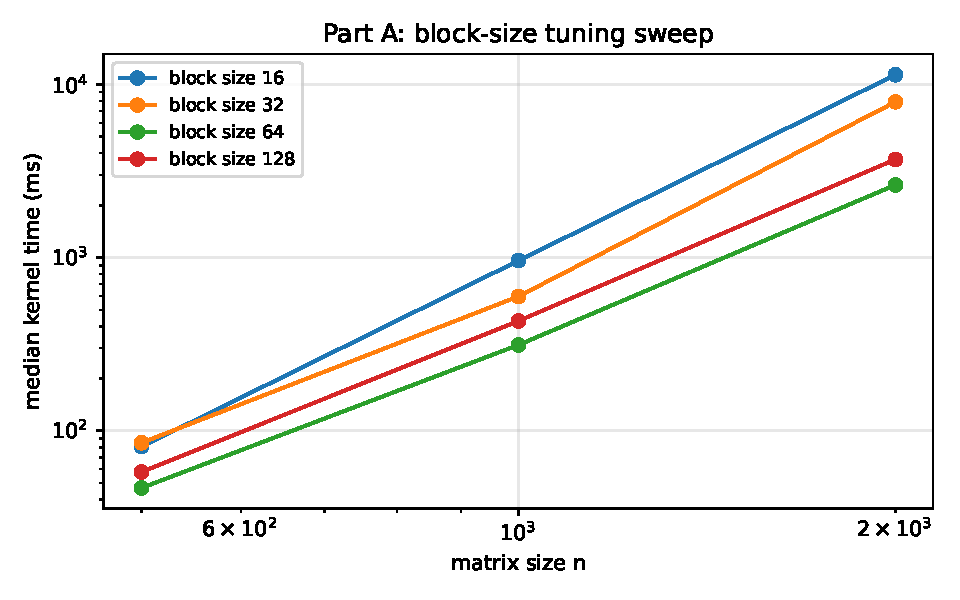
\includegraphics[width=0.78\textwidth]{fig3_blocksize.pdf}
\captionof{figure}{Tuning sweep of the block size. The 98\,KB working set of
$B=64$ (3 tiles of $64\times64$ doubles) matches the per-core L2 better than
the L1d-fitting $B=32$.}
\label{fig:tune}
\end{center}

\subsection{Part B: sparse multiplication at n = 1000}

\begin{table}[t]
\centering
\caption{Part B at $n=1000$: median kernel time (ms) per method and measured
nonzero count of $A$. The dense methods are flat in $p$; CSR tracks $nnz$.}
\label{tab:partB}
\small
\begin{tabular}{@{}rrrrrr@{}}
\toprule
sparsity & $nnz$ & \texttt{ijk} & \texttt{ikj} & \texttt{block} & \texttt{csr} \\
\midrule
1\,\%  & 989\,972 & 802  & 296 & 314 & \textbf{263} \\
5\,\%  & 949\,910 & 817  & 317 & 324 & \textbf{258} \\
10\,\% & 900\,120 & 813  & 271 & 322 & \textbf{250} \\
25\,\% & 749\,936 & 865  & 281 & 323 & \textbf{215} \\
50\,\% & 499\,827 & 773  & 298 & 335 & \textbf{145} \\
75\,\% & 249\,722 & 807  & 284 & 317 & \textbf{70.7} \\
90\,\% & 100\,375 & 782  & 313 & 312 & \textbf{33.4} \\
95\,\% & 50\,189  & 795  & 326 & 357 & \textbf{14.9} \\
99\,\% & 9\,844   & 810  & 357 & 348 & \textbf{4.0} \\
\bottomrule
\end{tabular}
\end{table}

Table~\ref{tab:partB} and Figure~\ref{fig:sparse} confirm H3 and H4: the three
dense methods vary by less than 12\,\% across the whole sparsity range (their
loops still touch every entry), while CSR falls monotonically from 263\,ms to
4.0\,ms. On this grid CSR is the fastest method at every sparsity level,
including 1\,\%, where it is already 1.1$\times$ faster than \texttt{ikj}; the
advantage grows to 25--90$\times$ at 90--99\,\% sparsity. The 2.4\,ms--10.7\,ms
dense-to-CSR conversion (Figure~\ref{fig:conv}) amortises after 0.07
multiplications at 50\,\% sparsity and after 0.01 at 90\,\%.

\begin{center}
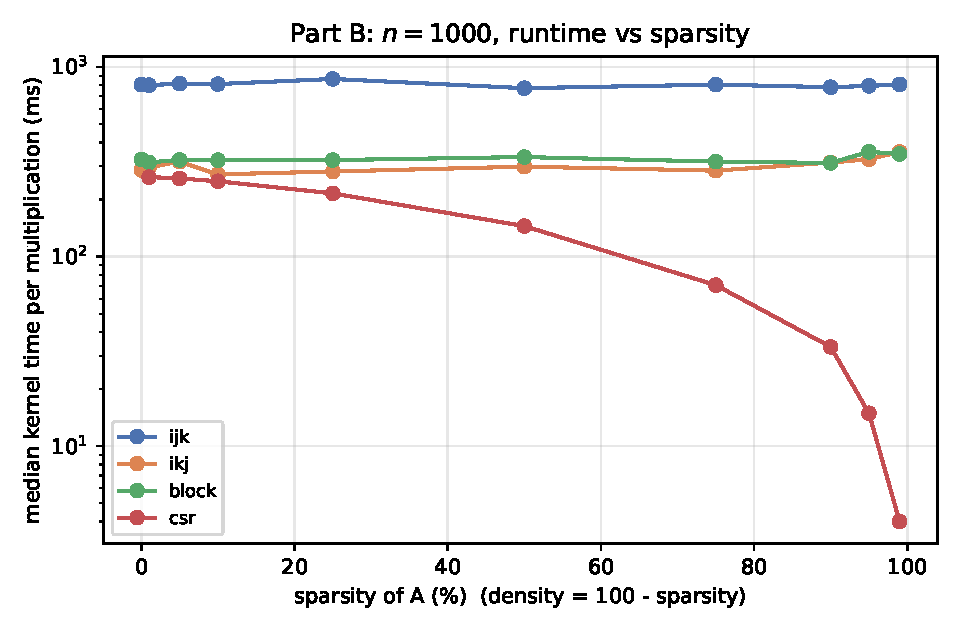
\includegraphics[width=0.82\textwidth]{fig4_sparse_runtime.pdf}
\captionof{figure}{Part B: median kernel time vs.\ sparsity at $n=1000$ (log
y-axis). Dense methods are flat; CSR follows the nonzero count.}
\label{fig:sparse}
\end{center}

\begin{center}
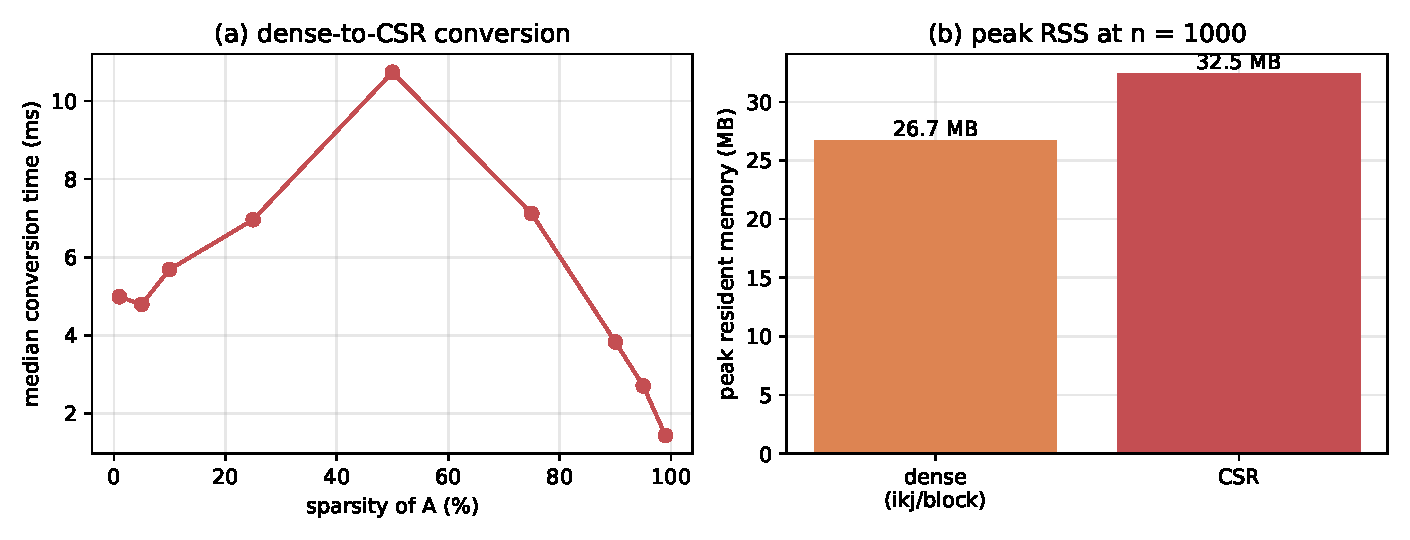
\includegraphics[width=0.95\textwidth]{fig5_conversion_memory.pdf}
\captionof{figure}{Part B: (a) median dense-to-CSR conversion time, measured
separately; (b) mean peak resident memory of the child at $n=1000$ (dense
methods vs.\ CSR).}
\label{fig:conv}
\end{center}

\subsection{Memory}

Peak resident memory at $n=1000$ is 26.7\,MB for the dense methods (theoretical
raw storage $3\times 8n^2 = 24$\,MB plus runtime overhead) and up to 38.1\,MB with
CSR: the sparse format adds the index and value arrays ($\approx 3 \times 4\,nnz$
bytes, plus the row pointer), i.e.\ about 11\,MB at 99\,\% density and
proportionally less as sparsity grows. No configuration came near the 4\,GiB
budget; the largest configuration ($n=2000$, \texttt{ijk}, 27.5\,s) stayed inside
the 60\,s budget, so the largest feasible tested size under the budget is
$n=2000$ for all three dense methods.

\section{Discussion}

\textbf{Part A.} H1 holds: reordering to \texttt{ikj} buys 2.5--2.8$\times$ at
medium sizes and 7$\times$ at $n=2000$, and the baseline's super-cubic local
exponent (4.26) is consistent with strided column reads of $B$ leaving cache and
TLB reach ($B$ is 32\,MB at $n=2000$ against a 12\,MB L3). H2 holds in the form
observed: blocking is pure overhead relative to \texttt{ikj} while the tiles fit
in cache anyway (up to $n=1000$), and only pays at $n=2000$, where the
$k$-tiling keeps 98\,KB working sets resident and restores near-cubic growth
(2.96). The tuning sweep supports the cache argument: $B=64$, whose three tiles
fit the 1.25\,MB L2, beat the L1d-fitting $B=32$ at every tuned size, and both
large candidates beat the too-small $B=16$.

\textbf{Part B.} H3 holds: on this machine the dense loops gain nothing from
zeros (a zero entry still costs a multiply and an add). H4 holds, with a
qualification: on the whole tested grid CSR wins already at 1\,\% sparsity, not
only at high sparsity. The reason visible in the kernel is locality, not just
arithmetic: CSR reads $A$ sequentially and streams $B$ and $C$ by rows, while even
the best dense method (\texttt{ikj}) still pays an $A[i][k]$ load and a strided
$k$ step per output element. The conversion that CSR requires is cheap
(1.4--10.7\,ms) and amortises within a single multiplication, so it never erases
the advantage at $n=1000$. H5 holds by construction and by measurement: all
checksums are bitwise identical.

\textbf{Methodological finding.} The discarded first campaign is itself a result:
on a hybrid laptop, the \emph{Balanced} power plan lets single-core frequency
swing by factors of 2--5 within one configuration, which would have corrupted
every cross-method comparison. Pinning and the \emph{High performance} plan (or
an equivalent fixed-frequency control) should be considered part of the
protocol on this class of machine.

\textbf{Limitations.}
\begin{enumerate}
  \item One machine, one compiler, sequential kernels only; the hybrid
        P/E core design means other laptops may rank the methods differently.
  \item Part~B tests a single size ($n=1000$); the dense-vs-CSR crossover is
        size-dependent and should not be extrapolated to $n=2000$ (CSR's memory
        traffic grows as $nnz \cdot n$, while blocked dense reuses cache).
  \item Sparsity is uniform random; clustered or structured sparsity can change
        CSR's row-length distribution and its performance. Percentage of zeros
        alone does not determine performance.
  \item All methods were auto-vectorised by the same compiler flags; no
        explicit vectorisation study was performed.
  \item Memory differences are working-set metrics of one process, not
        allocator-level breakdowns.
\end{enumerate}

Following the assignment guidance, the claims are limited to these
implementations, inputs and hardware~\cite{fleming1986,mytkowicz2009}.

\section{Conclusions}

Within the tested scope: (1) loop reordering to \texttt{ikj} is the reliable
winning optimisation for dense multiplication on this CPU, worth 2.5--7$\times$
over the validated \texttt{ijk} baseline; (2) cache blocking is not free --- it
loses to \texttt{ikj} up to $n=1000$ and wins only at $n=2000$, where the inputs
outgrow the last-level cache, with tile size 64 empirically best; (3) dense
runtimes are insensitive to sparsity, while CSR time tracks the nonzero count and
beats every dense method across all tested sparsity levels at $n=1000$, from
1\,\% to 99\,\% zeros; (4) CSR's conversion cost is negligible
($<0.1$ multiplications to amortise) and its memory overhead is about 11\,MB at
$n=1000$; and (5) power management, not algorithmics, was the dominant noise
source in the first campaign and had to be controlled explicitly.

Unresolved: the size dependence of the sparse crossover, structured sparsity,
and whether blocking and CSR compose (blocked CSR) or interact with the parallel
and distributed variants of Assignments~3 and~4.

\section{Reproducibility materials}

{\sloppy
All source code, shared inputs, raw measurements (CSV) and the executed analysis
notebook live in the public repository
\url{https://github.com/aledelgadoo/individual-assignments-bigdata};
the Git tag \texttt{assignment-2} marks the exact state submitted for this
assignment (the Assignment~1 baseline is preserved under tag
\texttt{assignment-1}). The \texttt{README.md} documents dependency versions and
the exact build, input-generation, benchmark, environment and analysis commands
that regenerate this report end to end.\par}

\section*{Generative-AI usage statement}

Following the course policy, the author discloses that the AI assistant
\textbf{opencode} (model \texttt{opencode/mimo-v2.6-flash-free}) was used, under
the author's direction, for planning the optimised kernels and the measurement
protocol, drafting and debugging parts of the C code and Python scripts,
generating the analysis notebook and figures, and revising the English of this
report. The author reviewed all generated code, executed and inspected the
correctness self-test, the tuning sweep, the benchmark campaign and every figure,
verified the numbers quoted here against the raw CSV files, and is responsible
for the measurements, the conclusions and any errors.

\begin{thebibliography}{9}
\bibitem{strang2016}
G. Strang, \emph{Introduction to Linear Algebra}, 5th ed.
Wellesley--Cambridge Press, 2016.

\bibitem{cormen2022}
T. H. Cormen, C. E. Leiserson, R. L. Rivest, and C. Stein,
\emph{Introduction to Algorithms}, 4th ed. MIT Press, 2022.

\bibitem{golub2013}
G. H. Golub and C. F. Van Loan, \emph{Matrix Computations}, 4th ed.
JHU Press, 2013.

\bibitem{saad2003}
Y. Saad, \emph{Iterative Methods for Sparse Linear Systems}, 2nd ed.
SIAM, 2003.

\bibitem{fleming1986}
W. P. Fleming and J. M. Wallace, ``How not to lie with statistics: the correct
way to summarize benchmark results,'' \emph{Communications of the ACM},
vol. 29, no. 3, pp. 218--221, 1986.

\bibitem{mytkowicz2009}
T. Mytkowicz, A. Diwan, M. W. Hauswirth, and P. F. Sweeney,
\emph{Measuring Computer Performance: A Practitioner's Guide}.
Cambridge University Press, 2009.

\bibitem{isoC11}
ISO/IEC 9899:2011, ``Information technology --- Programming languages --- C,''
International Organization for Standardization, 2011.

\bibitem{psutil}
G. Rodola, \emph{psutil: cross-platform process and system utilities}, 2026.
[Online]. Available: \url{https://github.com/giampaolo/psutil}
\end{thebibliography}

\end{document}
